\chapter{Drawing Graphs with Circular Arcs}
\label{chap:drawing-graphs-with-circular-arcs}

In the style of Schulz \cite{Schulz}, we shall now apply the concepts from \crefrange{chap:generalized-coordinates}{chap:minimizing-potential-energy} to create drawings of graphs with low visual complexity by drawing multiple incident edges using a single circular arc. The algorithms presented in this chapter allow us to create drawings of arbitrary connected and simple graphs. Potential edge crossings will be disregarded as they are unavoidable in nonplanar graphs and minimizing the number of edge crossings is generally ${\mathcal{NP}}$-hard.

\hfill

\noindent
Let ${\Pi = \left\lbrace P_1, \ldots, P_k \right\rbrace}$ be a set of edge-disjoint paths that may have vertices in common. We shall denote the entirety of vertices and edges of paths ${P \in \Pi}$ by ${V(\Pi)}$ and ${E(\Pi)}$, respectively:
%
\begin{align*}
  V(\Pi) &\coloneqq V(P_1) \cup \ldots \cup V(P_k)
  \\
  E(\Pi) &\coloneqq E(P_1) \cupplus \ldots \cupplus E(P_k)
\end{align*}






\noindent
Given a graph ${G = (V, E)}$, a \emph{drawing of ${G}$ with circular arcs} is a drawing of ${G}$ in which every edge ${e \in E}$ is drawn as a circular arc ${\Gamma_e}$, such that \begin{enumerate*}[label=(\roman*)] \item no vertices coincide, \item no edges overlap, and \item no edge intersects vertices other than its endpoints \end{enumerate*}. For the purpose of working with circular arcs only, we shall consider straight line segments to be circular arcs with infinite radius and complete circles to be circular arcs, too.

Similarly, given a set of edge-disjoint paths ${\Pi = \left\lbrace P_1, \ldots, P_k \right\rbrace}$, a \emph{drawing of ${\Pi}$ with circular arcs} is a drawing of the graph ${G \coloneqq (V(\Pi), E(\Pi))}$ with circular arcs, such that the edges of each path ${P \in \Pi}$ form a single circular arc ${\Gamma_P}$. Note that this does not violate above condition of every edge being drawn as a circular arc, since subdividing a circular arc yields other, though smaller, circular arcs. The fact that edges may not overlap implies that the order of vertices on ${\Gamma_P}$ must be as indicated by ${P}$.

The definition of a drawing of ${\Pi}$ with circular arcs \emdash and therefore ${\Pi}$ itself \emdash implicitly defines the constraints a drawing of ${\Pi}$ is subject to. Note that only the constraints of all vertices ${v \in V(P)}$ on a path ${P \in \Pi}$ lying on the same circular arc ${\Gamma_P}$ can be expressed as holonomic constraints. The constraints of said vertices having the correct order on ${\Gamma_P}$, no vertices coinciding, no edges overlapping, and no edge intersecting vertices other than its endpoints can not be expressed as holonomic constraints. These constraints do not reduce the number of degrees of freedom in the drawing \emdash they simply render some drawings invalid, but need to be accounted for nonetheless.



\clearpage
\section{Existence of Drawings with Circular Arcs}
\label{sect:existence-of-drawings-with-circular-arcs}

For an arbitrary set of edge-disjoint paths ${\Pi = \left\lbrace P_1, \ldots, P_k \right\rbrace}$ the existence of a drawing of ${\Pi}$ with circular arcs is not guaranteed.

A circle \emdash or circular arc for that matter \emdash is uniquely determined by three distinct points. If two paths ${P_i \neq P_j}$ were to have three or more vertices in common, the circular arcs used to draw them would intersect in at least three points and would therefore overlap. However, in \cref{thm:necessary-condition-not-sufficient} we show that the resulting necessary condition of two paths ${P_i \neq P_j}$ having at most two vertices in common is not sufficient in guaranteeing the existence of a (valid) drawing of ${\Pi}$ with circular arcs. We start by showing the following lemma:

\hfill



\begin{lemma}
\label{thm:existence-without-touches}
A drawing of ${\Pi}$ with circular arcs in which edges touch in non-endpoints can be transformed into a drawing of ${\Pi}$ with circular arcs in which said edges either cross or do not intersect at all.
\end{lemma}

\begin{proof}
When two edges touch in non-endpoints, then so do the paths they are part of and the circular arcs used to draw these paths. Adjusting the curvature of one of said circular arcs by an infinitesimal amount causes these circular arcs to either cross or to not intersect at all.

Considering this adjustment does not alter the ordering of vertices on said circular arc, it is only left to show that this adjustment can be performed such that the resulting circular arc does not overlap other circular arcs, or intersect vertices not part of the respective path. There's a finite number of vertices and paths in a drawing of ${\Pi}$ with circular arcs; hence this adjustment can indeed be performed without violating any of the constraints imposed by ${\Pi}$.
\end{proof}





\clearpage

\begin{theorem}
\label{thm:necessary-condition-not-sufficient}
There exists a set of edge-disjoint paths ${\Pi}$ in which any two paths have at most two vertices in common, \ie{} ${\forall i \neq j \colon \abs{V(P_i) \cap V(P_j)} \leq 2}$, for which no (valid) drawing with circular arcs exists.
\end{theorem}

\begin{proof}
An arrangement of pseudocircles is a finite list ${\mathcal{C} = (c_1, \ldots, c_n)}$ of Jordan curves in the plane, such that \begin{enumerate*}[label=(\roman*)] \item every two curves intersect in at most two points, and \item if two curves meet in a point, they cross in said point \end{enumerate*}. Two arrangements are said to be \emph{equivalent} if there exists a homeomorphism from the plane onto itself that transforms one of the arrangements into the other one. An arrangement of pseudocircles is said to be \emph{circleable} if it is equivalent to an arrangement of proper circles \cite{Kang}.

Linhart and Ortner \cite{Linhart} showed that the arrangement of pseudocircles in \cref{fig:non-circleable-arrangement-of-pseudocircles} is not circleable.

\begin{figure}[H]
  \centering
  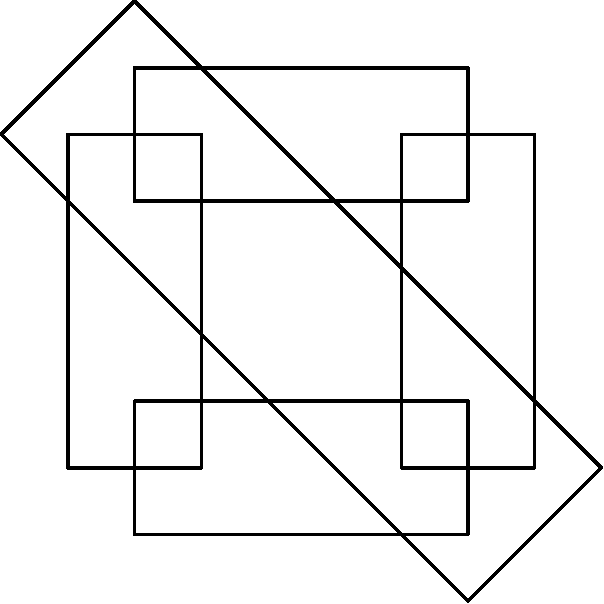
\includegraphics[width=0.4\textwidth]{Resources/Figures/Arrangement-of-Pseudocircles.pdf}
  \quad
  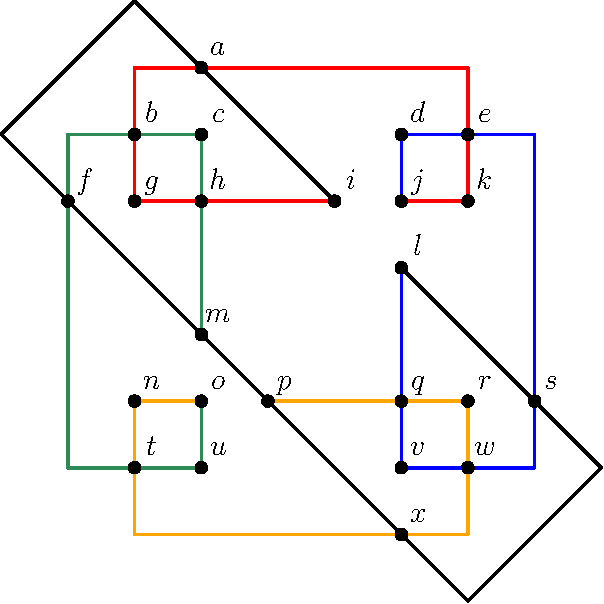
\includegraphics[width=0.4\textwidth]{Resources/Figures/Arrangement-of-Pseudoarcs.pdf}
  \caption{An arrangement of pseudocircles that is not circleable (left) and a derived arrangement of pseudo circular arcs (right).}
  \label{fig:non-circleable-arrangement-of-pseudocircles}
\end{figure}

\noindent
Let us choose a set of edge-disjoint paths ${\Pi = \lbrace P_1, \ldots, P_n \rbrace}$ such that each path represents one of the pseudocircles in \cref{fig:non-circleable-arrangement-of-pseudocircles} and their shared vertices completely encode all of said pseudocircles' intersections with each other. A possible choice would be ${P_1 = \mathit{ihgbaekj}}$ (red), ${P_2 = \mathit{pqrwxtno}}$ (yellow), ${P_3 = \mathit{mhcbftuo}}$ (green), ${P_4 = \mathit{lqvwsedj}}$ (blue), and ${P_5 = \mathit{iafmpxsl}}$ (black).

Considering circular arcs are slices of complete circles and the arrangement of pseudocircles in \cref{fig:non-circleable-arrangement-of-pseudocircles} is not circleable, a drawing of ${\Pi}$ with circular arcs in which no two circular arcs touch in non-endpoints can not exist. \Cref{thm:existence-without-touches} then shows that in fact, no drawing of ${\Pi}$ with circular arcs can exist at all.
\end{proof}





\clearpage

\noindent
\Cref{thm:necessary-condition-not-sufficient} shows that the trivial condition of two paths having at most two vertices in common is not sufficient in guaranteeing the existence of a (valid) drawing of ${\Pi}$ with circular arcs. Let us now be a little more restrictive and instead consider an ordered sequence of edge-disjoint paths ${\Pi = (P_1, \ldots, P_k)}$ in which none of a path ${P_i}$'s internal vertices are contained in an earlier path, \ie{} a path ${P_j}$ with ${j < i}$:
%
\begin{equation}
  V_\text{int}(P_i) \cap V(P_1 \cup \ldots \cup P_{i-1}) \stackrel{!}{=} \varnothing,
  \quad i = 2 \ldots k
  \label{eqn:blah-blah-property}
\end{equation}





\hfill

\begin{theorem}
\label{thm:existence-of-drawing}
An ordered sequence of edge-disjoint paths ${\Pi = (P_1, \ldots, P_k)}$ fulfilling \cref{eqn:blah-blah-property} permits a drawing of ${\Pi}$ with circular arcs.
\end{theorem}

\begin{proof}
We will provide a method to construct a drawing of ${\Pi}$ with circular arcs by sequentially drawing the paths ${P \in \Pi}$ in their designated order.

\Cref{eqn:blah-blah-property} ensures that, when drawing a path ${P = (v_1, \ldots, v_n)}$, its internal vertices ${v_2, \ldots, v_{n-1}}$ have not yet been drawn. Since the paths are edge-disjoint, its edges have not yet been drawn either. In case an endpoint of ${P}$ has not yet been drawn, we can assign it an arbitrary position, as long as it is not on any of the circular arcs that have already been drawn.

Considering there's a finite number of vertices and edges, there exists a circular arc ${\Gamma_P}$ between ${P}$'s endpoints that neither intersects any of the vertices that have already been drawn (other than said endpoints), nor overlaps any circular arc that has already been drawn.

It is possible, however, for ${\Gamma_P}$ to intersect other circular arcs. Drawing one of ${P}$'s internal vertices on such an intersection would visually introduce new edges, rendering the drawing of ${\Pi}$ invalid. Considering a pair of non-overlapping circular arcs intersects in at most two points, the number of points on ${\Gamma_P}$ on which we can not draw ${P}$'s internal vertices is finite, and there are infinitely many points left on which said vertices could be drawn without rendering the drawing invalid. Therefore we can draw ${P}$'s internal vertices, in order, on the circular arc and thereby partition ${\Gamma_P}$ into smaller circular arcs ${\Gamma_e}$ representing the individual edges ${e \in E(P)}$.
\end{proof}





\hfill

\noindent
We have seen that an ordered sequence of edge-disjoint paths ${\Pi = (P_1, \ldots, P_k)}$ fulfilling \cref{eqn:blah-blah-property} permits a (greedy) drawing of ${\Pi}$ with circular arcs. Therefore we shall also refer to ${\Pi}$ as a \emph{greedily realizable sequence of paths}. Vertices ${v \in V(\Pi)}$ shall be said to be \emph{laid out} by the first path, \ie{} the path ${P_i \in \Pi}$ with the lowest index ${i}$, in which they occur. If ${v}$ is internal to said path, it shall be called \emph{constrained} (with respect to ${\Pi}$); otherwise, it shall be called \emph{unconstrained} (with respect to ${\Pi}$). The constrained and unconstrained vertices form the sets ${V_\text{c}(\Pi)}$ and ${V_\text{u}(\Pi)}$, respectively. Obviously ${V_\text{c}(\Pi) \cap V_\text{u}(\Pi) = \varnothing}$ and ${V_\text{c}(\Pi) \cup V_\text{u}(\Pi) = V(\Pi)}$.

Note that there are definitely other properties guaranteeing the existence of a (valid) drawing of ${\Pi}$ with circular arcs \emdash possibly even less restrictive ones. We use this one because it suggests a straight-forward method to create a drawing, as illustrated in the proof of \cref{thm:existence-of-drawing}.


\clearpage
\section{Graph Decomposition}
\label{sect:graph-decomposition}

In this section, we shall discuss a generic approach to decompose a connected and simple graph into a non-trivial greedily realizable sequence of simple paths. We restrain ourselves to connected graphs since paths can not contain isolated vertices. Besides, in a larger graph, the connected components can \emdash and should \emdash be drawn individually. The graph being simple allows it to be decomposed into simple paths, which will be a requirement in a later section.

\Cref{algo:greedy-graph-decomposition} greedily assembles the paths one after the other.
The \code{vertices} and \code{edges} sets keep track of which vertices and edges have already been used and allow us to ensure that the assembled paths both are edge-disjoint and fulfill \cref{eqn:blah-blah-property}.

\hfill

\begin{algorithm}[H]
  \caption{Graph Decomposition}
  \label{algo:greedy-graph-decomposition}
  \SetKw{Break}{break}
  \SetKw{Continue}{continue}
  \SetKw{Ensure}{ensure}
  \SetKwData{Paths}{paths}
  \SetKwData{Vertices}{vertices}
  \SetKwData{Edges}{edges}
  \SetKwData{Path}{path}
  \SetKwData{Head}{head}
  \SetKwFunction{Append}{append}
  \SetArgSty{textrm}
  \vspace{5pt}
  \KwData{Connected and simple graph ${G}$}
  \KwResult{Greedily realizable sequence of simple paths ${\Pi}$, such that ${V(\Pi) = V(G)}$ and ${E(\Pi) = E(G)}$}
  \vspace{10pt}
  ${\Paths \gets ()}$\;
  ${\Edges \gets \varnothing}$\;
  ${\Vertices \gets \varnothing}$\;
  \;
  \ForEach{${u \in V(G)}$}{
    \label{line:decomposition-choose-vertex}
    \ForEach{${e = \lbrace u, v \rbrace \in E(G)}$}{
      \label{line:decomposition-choose-first-edge}
      \Ensure{${e \notin \Edges}$} \lElse{\Continue}
      \;
      ${\Path \gets (e)}$\;
      ${\Head \gets v}$\;
      ${\Edges \gets \Edges \cupplus \lbrace e \rbrace}$\;
      ${\Vertices \gets \Vertices \cup \lbrace u \rbrace}$\;
      \;
      append:\;
      \label{line:decomposition-append-loop}
      \While{${\Head \notin \Vertices}$}{
        ${\Vertices \gets \Vertices \cupplus \lbrace \Head \rbrace}$\;
        \label{line:decomposition-append-loop-once-per-vertex}
        \;
        \ForEach{${f = \lbrace \Head, w \rbrace} \in E(G)$}{
          \label{line:decomposition-choose-next-edge}
          \Ensure{${f \notin \Edges}$} \lElse{\Continue}
          \Ensure{${w \notin \Path.\Vertices}$} \lElse{\Continue}
          \label{line:decomposition-ensure-simple-paths}
          \;
          ${\Path \gets \Path.\Append{f}}$\;
          ${\Head \gets w}$\;
          ${\Edges \gets \Edges \cupplus \lbrace f \rbrace}$\;
          \;
          \Continue append \;
        }
        \Break\;
      }
      ${\Paths \gets \Paths.\Append{\Path}}$\;
    }
  }
  \;
  \Return ${\Paths}$
\end{algorithm}
\vspace*{\fill}



\paragraph{Correctness}

After the loop in \cref{line:decomposition-choose-first-edge}, all edges incident to ${u}$ are guaranteed to appear in a path. Because this loop is executed for every vertex in the input graph ${G}$, all edges in the graph end up being used. By definition the input graph is connected; hence every vertex is incident to at least one edge, meaning that all vertices in the graph are used as well. Considering that edges are only ever used to assemble the working path if they have not been used before, we find that ${\Pi}$ is a decomposition of the input graph, \ie{} ${V(\Pi) = V(G)}$ and ${E(\Pi) = E(G)}$.

It remains to show that ${\Pi}$ is a greedily realizable sequence of simple paths. Since the input graph does not contain loops, a single edge always is a simple path. Single-edged paths cannot possibly violate the requirements of a greedily realizable sequence of paths, as they do not have any internal vertices that could have appeared in an earlier path. When appending an edge to the working path, its current head would become an internal vertex. This operation is only performed if the current head can become an internal vertex without violating the requirements in \cref{eqn:blah-blah-property}, \ie{} if the current head has not been used beforehand. The additional check in \cref{line:decomposition-ensure-simple-paths} ensures that edges are only appended to the working path if the resulting path would still be simple, \ie{} if appending the edge would not form a cycle. Therefore ${\Pi}$ is indeed a greedily realizable sequence of simple paths.



\paragraph{Runtime}

The two outermost loops iterate over all vertices and their incident edges. Considering an edge is incident only to its endpoints, each edge is processed exactly twice here. When implemented using an adjacency list, these loop conditions can be checked in ${\bigTheta{\abs{V} + \abs{E}}}$.

The condition of the \code{append} loop in \cref{line:decomposition-append-loop} is checked ${\bigTheta{\abs{V} + \abs{E}}}$ times as a result of the containing loop being executed that many times; plus once whenever the algorithm jumps back to the \code{append} label after appending an edge to the working path, which happens ${\bigOh{\abs{E}}}$ times. \Cref{line:decomposition-append-loop-once-per-vertex} ensures that the loop's body, however, is executed at most once per vertex. Using the same argument as above, iterating over the incident edges of ${\bigOh{\abs{V}}}$ vertices can be done in ${\bigOh{\abs{V} + \abs{E}}}$.

As a result, the entire algorithm can be executed in ${\bigTheta{\abs{V} + \abs{E}}}$ when implemented using an adjacency list.



\paragraph{Adaptation}

The sole purpose of above algorithm is to show that it is relatively easy to decompose an input graph ${G}$ into a non-trivial greedily realizable sequence of paths ${\Pi}$ using a greedy algorithm. It does not intend to find a \emph{good} decomposition \emdash quality is a subjective measurement and very much depends on what one wants to achieve when drawing the graph.

Possible tweaks include the choice of vertices in \cref{line:decomposition-choose-vertex} or the choice of edges in \cref{line:decomposition-choose-first-edge} and \cref{line:decomposition-choose-next-edge}. It may even be an option to not greedily append edges as long as possible, and instead start a new path earlier, especially in undirected graphs. In a directed graph, for example, it would make sense to keep track of the number of unused incoming edges for each vertex and pick a vertex with no unused incoming edges in \cref{line:decomposition-choose-vertex}.

It may also be useful to let the user, who possibly has background knowledge about what the graph represents, provide some paths that semantically make sense to emphasize by drawing them as a single circular arc. The user-provided paths can then be completed to a valid decomposition ${\Pi}$ of the input graph.


\clearpage
\section{Circular Arc Geometry}
\label{sect:circular-arc-geometry}

A 3-tuple ${(P, Q, \varphi)}$ uniquely determines a circular arc ${\Gamma(P, Q, \varphi)}$. Here ${P, Q \in \mathbb{R}^2}$ are its distinct endpoints, and ${\varphi \in (-180\degrees, 180\degrees)}$ is the (signed) angle from the chord ${PQ}$ to the arc's tangent in ${P}$.

Drawing a circular arc with ${\varphi > 0 \degrees}$ starting in ${P}$ requires a clockwise motion; hence those arcs shall be called \emph{clockwise}. Similarly, arcs shall be called \emph{counterclockwise} for ${\varphi < 0 \degrees}$. For ${\varphi = 0 \degrees}$ the arc degenerates into the straight line segment connecting ${P}$ and ${Q}$. \Cref{fig:circular-arc-geometry} outlines important properties of a circular arc.
%
\begin{figure}[H]
  \centering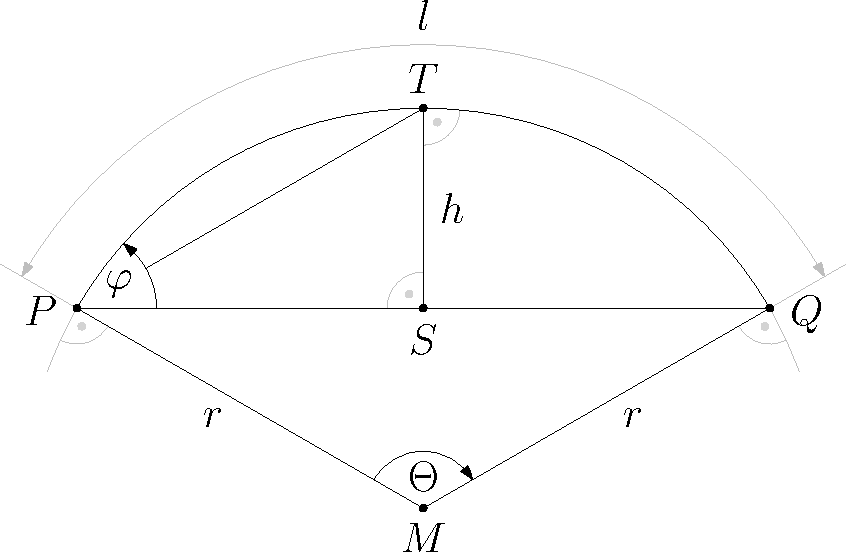
\includegraphics[width=0.6\textwidth]{Resources/Figures/Clockwise-Circular-Arc.pdf}
  \caption{Geometry of a clockwise circular arc.}
  \label{fig:circular-arc-geometry}
\end{figure}



\noindent
The \emph{central angle} ${\Theta}$ is the (signed) angle which the arc subtends at the center of the circle. For clockwise arcs the central angle is negative; for counterclockwise arcs it is positive:
%
\begin{equation*}
  \Theta = -2 \varphi
\end{equation*}



\noindent
The \emph{arc height} ${h}$ is the (signed) perpendicular distance from the arc's midpoint ${T}$ to the chord ${PQ}$ connecting its endpoints. For clockwise arcs the arc height is positive; for counterclockwise arcs it is negative. When cutting ${\Gamma}$ in half, the circular arc ${\Gamma'}$ with chord ${PT}$ has ${\Theta' = \frac{\Theta}{2}}$ and ${\varphi' = \frac{\varphi}{2}}$. Therefore we find ${\angle SPT = \varphi - \frac{\varphi}{2}}$, and we can write the arc height as
%
\begin{equation*}
  h \: = \: \segment{PS} \cdot \eval{\tan}{\angle SPT} \; = \; \frac{1}{2} \segment{PQ} \cdot \eval{\tan}{\frac{\varphi}{2}}.
\end{equation*}



\noindent
The \emph{arc radius} ${r}$ and \emph{arc center} ${M}$ are, respectively, the radius and center of the circle which the arc is a slice of. We find them to be
%
\begin{align*}
  r(\varphi \neq 0 \degrees) &= \abs{\frac{\segment{PS}}{\eval{\sin}{\varphi}}} = \abs{\frac{\segment{PQ}}{2 \eval{\sin}{\varphi}}}
  \intertext{and}
  M(\varphi \neq 0 \degrees) &= P + R(\varphi - 90 \degrees)
    \cdot \frac{\longvec{PQ}}{2 \eval{\sin}{\varphi}},
\end{align*}
%
where ${R(\psi)}$ is the matrix rotating a column vector by ${\psi}$ in the counterclockwise direction. Note that for ${\varphi = 0 \degrees}$, both radius ${r}$ and center ${M}$ are undefined.



The \emph{arc length} ${l}$ is the distance between the arc's endpoints ${P}$ and ${Q}$ along the arc. It is a portion of the respective circle's circumference:
%
\begin{equation*}
  l(\varphi \neq 0 \degrees) = \abs{\frac{\Theta}{360 \degrees} \cdot 2 \pi r} = \abs{\frac{\varphi}{180 \degrees} \cdot \frac{\pi \cdot \segment{PQ}}{\eval{\sin}{\varphi}}}
\end{equation*}



\noindent
For ${\varphi = 0 \degrees}$, above equation for arc length ${l}$ is undefined. We shall continuously extend it to ${\varphi = 0 \degrees}$ using the limit ${\lim_{\varphi \to 0 \degrees}}$:
%
\begin{equation*}
  l(\varphi = 0 \degrees) \coloneqq \lim_{\varphi \to 0 \degrees} l(\varphi) = \segment{PQ}
\end{equation*}
%
This extension also matches our intuition of the arc degenerating into a straight line segment for ${\varphi \to 0 \degrees}$.


\clearpage
\section{Generalized Coordinates}
\label{sect:generalized-coordinates}

Given a greedily realizable sequence of simple paths ${\Pi = (P_1, \ldots, P_k)}$, we shall now choose generalized coordinates such that the holonomic constraints defined by ${\Pi}$ are implicitly satisfied. The generalized coordinates introduced here require a circular arc's endpoints to differ and can therefore not be applied to paths whose endpoints coincide.

\hfill

\noindent
Besides its endpoints, a circular arc requires another generalized coordinate encoding its curvature for it to be uniquely determined. This coordinate must be able to encode the arc's direction, \ie{} whether it is drawn clockwise or counterclockwise. Considering two circular arcs with the same angle $\varphi$, as introduced in the previous section, are guaranteed to be similar, we shall use the angle ${\varphi_P \in (-180 \degrees, 180 \degrees)}$ as a generalized coordinate encoding the curvature of the circular arc ${\Gamma_P}$.

Unconstrained vertices ${v \in V_\text{u}(\Pi)}$ can move around arbitrarily and require two degrees of freedom. We shall use Cartesian coordinates ${(x_v, y_v) \in \mathbb{R}^2}$ to represent their positions.

In contrast, constrained vertices ${v \in V_\text{c}(\Pi)}$ can not move around arbitrarily \emdash they are each being laid out by a path ${P(v)}$ and are restricted to move along the circular arc ${\Gamma_{P(v)}}$, while also staying in the order indicated by ${P(v)}$. We only have one degree of freedom per vertex here: its relative progress along the arc. It can be encoded using a generalized coordinate ${p_v \in (0, 1)}$ specifying the proportion of the subarc connecting ${P(v)}$'s tail and ${v}$ to the entire arc, as illustrated in \cref{fig:generalized-coordinates-for-single-path}.



\hfill
\begin{figure}[H]
  \centering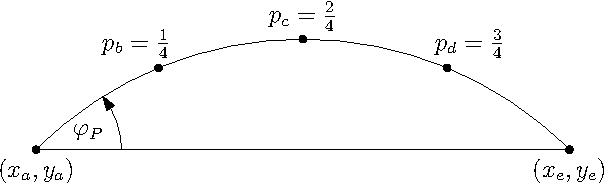
\includegraphics[width=0.7\textwidth]{Resources/Figures/Generalized-Coordinates-Example.pdf}
  \caption{Generalized coordinates for a single path ${P = abcde}$ with equi-length edges.}
  \label{fig:generalized-coordinates-for-single-path}
\end{figure}
\clearpage



\noindent
Collectively, the ${\bigTheta{\abs{V} + \abs{\Pi}}}$ generalized coordinates uniquely determine all of the vertices' positions ${\vec{r}_v}$ and circular arcs ${\Gamma_P}$. We shall write them as a 4-tuple ${q_{_\Pi} = (x, y, \varphi, p)}$, where
%
\begin{alignat*}{3}
  x & \colon & V_\text{u}(\Pi) &\to \mathbb{R},\\
  y & \colon & V_\text{u}(\Pi) &\to \mathbb{R},\\
  \varphi & \colon & \phantom{V_\text{u}(}\Pi\phantom{)} &\to (-180 \degrees, 180 \degrees),\\
  p & \colon & V_\text{c}(\Pi) &\to (0, 1).
\end{alignat*}

\noindent
The generalized coordinates chosen here satisfy all holonomic constraints defined by ${\Pi}$, \ie{} all vertices ${v \in V(P)}$ on a path ${P \in \Pi}$ are guaranteed to lie on the same circular arc $\Gamma_P$.

Recall that the configurations that can be expressed only depend on the constraints implicitly satisfied by the choice of generalized coordinates, and that the number of independent generalized coordinates equals the number of degrees of freedom in the system. It is therefore not possible to use fewer generalized coordinates while satisfying the same constraints without also excluding other configurations.


\clearpage
\section{Transformation of Generalized Coordinates}
\label{sect:transformation-of-generalized-coordinates}

Although generalized coordinates ${q_{_\Pi}}$ are helpful as an internal representation that implicitly satisfies the holonomic constraints, we will need to retrieve vertices' positions ${\vec{r}_v}$ and circular arcs ${\Gamma_P}$ to eventually produce a drawing of the graph ${G \coloneqq (V(\Pi), E(\Pi))}$.


In theory, we can write both the position vectors ${\vec{r}_v}$ and circular arcs ${\Gamma_P}$ as an explicit function of the generalized coordinates. However, these expressions get out of hand very quickly when paths are nested within one another, \ie{} a path's internal vertex is an endpoint of another path. Instead, we propose the following algorithm to perform the transformation to position vectors sequentially:

\bigskip

\begin{algorithm}[H]
  \caption{Transformation of generalized coordinates}
  \label{algo:transformation-of-generalized-coordinate}
  \SetKwData{Arc}{arc}
  \SetKwData{CircularArc}{CircularArc}
  \SetKwData{PointForProgress}{pointForProgress}
  \SetArgSty{textrm}
  \vspace{5pt}
  \KwData{Greedily realizable sequence of simple paths ${\Pi}$ and corresponding generalized coordinates ${q_{_\Pi} = (x, y, \varphi, p)}$, \ie{}
    \vspace{-8pt}
    \begin{flalign*}
      x \colon V_\text{u}(\Pi) &\to \mathbb{R},&\\
      y \colon V_\text{u}(\Pi) &\to \mathbb{R},&\\
      \varphi \colon \phantom{V_\text{u}(}\Pi\phantom{)} &\to (-180 \degrees, 180 \degrees),&\\
      p \colon V_\text{c}(\Pi) &\to (0, 1)&
    \end{flalign*}
  }
  \vspace{-4pt}
  \KwResult{Positions ${\vec{r}(v)}$ and arcs ${\Gamma(P)}$ for all vertices and paths in ${\Pi}$}
  \vspace{5pt}
  Initialize ${\vec{r} \colon V(\Pi) \to \mathbb{R}^2}$\;
  Initialize ${\Gamma \colon \Pi \to \CircularArc}$\;
  \;
  \ForEach{${v \in V_\text{u}(\Pi)}$}{
    \label{line:transformation-unconstrained-start}
    ${\vec{r}(v) \gets (x({v}), y({v}))}$\;
    \label{line:transformation-unconstrained-end}
  }
  \;
  \ForEach{${P = (v_1, \ldots, v_n) \in \Pi}$}{
    \label{line:transformation-constrained-start}
    \label{line:transformation-access-endpoints}
    ${\Arc \gets \CircularArc(\vec{r}(v_1), \vec{r}(v_n), \varphi(P))}$\;
    \;
    \ForEach{${v \in (v_2, \ldots, v_{n-1})}$}{
      ${\vec{r}(v) \gets \Arc.\PointForProgress(p(v))}$\;
    }
    \;
    ${\Gamma(P) \gets \Arc}$\;
    \label{line:transformation-constrained-end}
  }
  \;
  \Return $(\vec{r}, \Gamma)$
\end{algorithm}

\clearpage



\paragraph{Correctness}

In \crefrange{line:transformation-unconstrained-start}{line:transformation-unconstrained-end}, we determine the position vectors for unconstrained vertices ${v \in V_\text{u}(\Pi)}$. For those and only those the generalized coordinates ${x(v)}$, ${y(v)}$ are defined, and it is trivial to assemble the vertices' position vectors.

In \crefrange{line:transformation-constrained-start}{line:transformation-constrained-end}, the position vectors of constrained vertices ${v \in V_\text{c}(\Pi)}$ are determined. When constructing a circular arc ${\Gamma_P}$, we need to know its endpoints' positions. If an endpoint is unconstrained, then it had its position assigned already in \crefrange{line:transformation-unconstrained-start}{line:transformation-unconstrained-end}. If it is not, then it must be constrained, and by definition, it has appeared in an earlier path in whose iteration it had its position assigned. Therefore the endpoints' positions are well-defined at the time of access in \cref{line:transformation-access-endpoints}. Considering a path's internal vertices ${v}$ are constrained by \cref{eqn:blah-blah-property}, the ${p(v)}$ are well-defined, allowing us to compute the vertices' positions on ${\Gamma_P}$. \Cref{eqn:blah-blah-property} also guarantees that vertices do not appear as internal vertices to any more paths once laid out, and therefore have a position assigned only once.

Considering the position vectors are computed for both constrained and unconstrained vertices, all vertices ${v \in V(\Pi)}$ have their position assigned.



\paragraph{Runtime}

The partition of ${V(\Pi)}$ into ${V_\text{u}(\Pi)}$ and ${V_\text{c}(\Pi)}$ is implicitly given by the domain of ${x}$, ${y}$, and ${p}$. Therefore \crefrange{line:transformation-unconstrained-start}{line:transformation-unconstrained-end} can be implemented in ${\bigTheta{\abs{V_\text{u}(\Pi)}}}$. In \crefrange{line:transformation-constrained-start}{line:transformation-constrained-end}, we construct a circular arc for each path ${P \in \Pi}$ and use it to compute the positions of ${P}$'s internal vertices in ${\bigTheta{1}}$ each. Considering each vertex ${v \in V_\text{c}(\Pi)}$ has its position assigned once and once only, \crefrange{line:transformation-constrained-start}{line:transformation-constrained-end} run in ${\bigTheta{\abs{\Pi} + \abs{V_\text{c}(\Pi)}}}$, yielding a total runtime of ${\bigTheta{\abs{\Pi} + \abs{V(\Pi)}}}$, which is optimal.



\paragraph{Validity of Drawings}

The drawing the algorithm produces is not necessarily a (valid) drawing of ${\Pi}$ with circular arcs. While the generalized coordinates implicitly satisfy the constraints of all vertices on a path ${P}$ lying on the same circular arc ${\Gamma_P}$, they do not make any guarantees about vertices not coinciding, edges not overlapping, or edges intersecting no vertices other than their endpoints. Recall that if the order of vertices on ${\Gamma_P}$ is not as indicated by ${P}$, then there inevitably are overlapping edges. These constraints will be dealt with in the following section.


\clearpage
\section{Forces and Potential Energy}
\label{sect:forces-and-potential-energy}

Let ${G = (V, E)}$ be a connected and simple input graph. We have seen that one can efficiently decompose ${G}$ into a greedily realizable sequence of simple paths ${\Pi = (P_1, \ldots, P_k)}$ and choose generalized coordinates that implicitly satisfy the holonomic constraints defined by ${\Pi}$.

For a configuration ${q_{_\Pi}}$ to yield a valid drawing of the graph, it is left to ensure that no vertices coincide, that no edges overlap, and that no edge intersects any vertices other than its endpoints. By assigning each configuration a potential energy that is finite if and only if said constraints are satisfied, we can easily distinguish valid from invalid drawings. This potential energy also serves as a measurement of the resulting drawing's quality and can be optimized to get better-looking drawings of ${G}$.

When drawing a graph, we want the vertices to be well spaced out with adjacent vertices being close together. Defining both attractive and repulsive forces between each pair of vertices is a standard procedure in many force-directed algorithms \cite{Kobourov} and can be applied here as well. In a mechanical system, the forces would act on the vertices and move them around to decrease the implicitly defined potential energy of the system.

In the following, ${c_i \in (0, \infty)}$ are constants used to scale various physical quantities.





\paragraph{Vertex-Vertex Repulsion}

Thinking of the vertices as charged particles pushing each other away allows us to space them out. A repulsive force ${F_\text{rep}}$ based on Coulomb's law attempts to push two vertices away from each other. It is exerted along the line connecting the vertices, and its magnitude depends on their distance ${d}$:
%
\begin{equation*}
  F_\text{rep}(d) \coloneqq c_1 \cdot \frac{1}{d^2}
\end{equation*}
%
We can write the electric potential energy stored in such a pair of charged particles as
%
\begin{align*}
  U_\text{rep}(u, v) \coloneqq{}& \int\limits_{\infty}^{\mathclap{d(u, v)}} -F_\text{rep}(s) \differential{s}
  \\
  ={}& c_1 \cdot \frac{1}{d(u, v)},
\end{align*}
%
where ${d(u, v)}$ is the Euclidean distance of the vertices ${u}$ and ${v}$'s positions. For ${d(u, v) = 0}$ the constraint of vertices not coinciding is violated, and we shall define ${U_\text{rep}(u, v) \coloneqq \infty}$.





\paragraph{Vertex-Vertex Attraction}

In order to keep adjacent vertices close together, we think of every edge as a virtual spring attempting to restore its relaxed length ${k}$. Linear springs based on Hooke's law have shown to be too strong when adjacent vertices are far away from each other. Therefore we shall use springs whose restoring forces ${F_\text{att}}$ are instead logarithmic in their relative displacement:
%
\begin{equation*}
  F_\text{att}(l) \coloneqq -c_2 \cdot k \cdot \eval{\ln}{\frac{l}{k}}
\end{equation*}
%
The elastic potential energy stored in such a spring can be written as
%
\begin{align*}
  U_\text{att}(e) \coloneqq{}& \int\limits_{k}^{\mathclap{l(\Gamma_e)}} -F_\text{att}(s) \differential{s}
  \\
  ={}& c_2 \cdot kl \cdot \left( \eval{\ln}{\frac{l}{k}} - 1 \right) + k^2,
\end{align*}
%
where ${\Gamma_e}$ is the circular arc used to draw the edge ${e}$, and ${l(\Gamma_e)}$ is its arc length.





\paragraph{Overlapping Edges}

Edges can overlap either within a single path or between two distinct paths. For each path ${P \in \Pi}$ we can define a potential energy that is zero if no edges ${e \in E(P)}$ overlap each other, and infinite otherwise:
%
\begin{equation*}
  U_\text{ord}(P) \coloneqq \begin{cases}
    0 & \text{if edges ${e \in E(P)}$ do not overlap}
    \\
    \infty & \text{otherwise}
  \end{cases}
\end{equation*}
%
If edges within a path overlap, its internal vertices are not ordered correctly on the circular arc ${\Gamma_P}$. In the process of transferring vertices from being ordered correctly to being ordered incorrectly, two vertices ${u \neq v}$ must coincide, \ie{} ${d(u,v) = 0}$, for which ${U_\text{rep}(u,v) = \infty}$. Therefore ${U_\text{ord}}$ does not affect the continuity or local differentiability of the total energy function. Overlapping edges of different paths will be dealt with in the next paragraph.





\paragraph{Vertex-Path Repulsion}

Edges of different paths ${P_i \neq P_j}$ can only overlap if the two circular arcs ${\Gamma_{P_i}}$, ${\Gamma_{P_j}}$ overlap. This case only occurs if at least one of the paths' endpoints lies on the other arc. Since the input graph ${G}$ is simple, this is equivalent to a circular arc intersecting vertices its respective path does not contain.

Therefore it is sufficient to ensure that vertices ${v}$ only lie on those circular arcs ${\Gamma_P}$ where they are part of the respective path, \ie{} ${v \in V(P)}$. For each path ${P \in \Pi}$ and vertex ${v \notin V(P)}$, we can define another potential energy that is finite if and only if ${v}$ does not lie on ${\Gamma_P}$ as
%
\begin{equation*}
  U_\text{int}(v, P) \coloneqq \begin{cases}
    c_3 \cdot \frac{1}{d(v, \Gamma_P)} & \text{if}~d(v, \Gamma_P) \neq 0
    \\
    \infty & \text{otherwise.}
  \end{cases}
\end{equation*}
%
Here ${d(v, \Gamma_P)}$ is the minimum Euclidean distance from the vertex ${v}$'s position to any point on the circular arc ${\Gamma_P}$. Note that by defining the potential energy, the corresponding restoring force is implicitly defined as well.





\paragraph{Total Potential Energy}

Using the four components described above, we can now calculate the total potential energy of the system determined by a configuration ${q_{_\Pi}}$:
%
\begin{equation*}
  U(q_{_\Pi}) \coloneqq
  \sum_{\mathclap{\substack{\lbrace u, v \rbrace \in V^2}}} U_\text{rep}(u, v)
  +
  \sum_{\mathclap{\substack{e \in E}}} U_\text{att}(e)
  +
  \sum_{\mathclap{\substack{P \in \Pi}}} U_\text{ord}(P)
  +
  \sum_{\mathclap{\substack{v \in V, P \in \Pi \\ v \notin V(P)}}} U_\text{int}(v, P)
\end{equation*}

\noindent
The summands \emdash and therefore their sum, too \emdash are finite if and only if all the constraints defined by ${\Pi}$ are satisfied. Thus we can easily tell whether or not a configuration yields a (valid) drawing of ${\Pi}$ with circular arcs by calculating the system's total potential energy. The energy function can be evaluated in ${\bigOh{\abs{V}^2 + \abs{E} + \abs{V} \cdot \abs{\Pi}}}$ time.





\hfill

\hiddensubsection{Minimizing Potential Energy}

Considering an explicit function for the ${\vec{r}_v}$ is not feasible as illustrated in \cref{sect:transformation-of-generalized-coordinates}, closed-form expressions for the forces or the system's total potential energy are not feasible either. It is therefore not an option to use generalized forces to minimize the system's potential energy; let alone to perform an analytical optimization. Instead, we shall resort to a generic hill climbing algorithm to find a local energy minimum.

Since hill climbing generally works on real-valued functions of ${n}$ variables, we need the total energy function to be of the form ${U \colon \mathbb{R}^n \to \mathbb{R} \cup \lbrace\infty\rbrace}$. The following bijective transformations allow all generalized coordinates to be used as real numbers and vice versa:
%
\begin{align*}
  (-180 \degrees, 180 \degrees) \ni \varphi & \mapsto c_4 \cdot \eval{\tan}{\frac{\varphi}{2}} \in \mathbb{R}
  \\
  (0, 1) \ni p & \mapsto c_5 \cdot \eval{\tan}{\pi \cdot (p - 0.5)} \in \mathbb{R}
\end{align*}


\noindent
We can then collect all ${n}$ generalized coordinates in a real-valued vector ${q \in \mathbb{R}^n}$ determining the system's configuration and evaluate its potential energy in ${\bigOh{\abs{V}^2 + \abs{E} + \abs{V} \cdot \abs{\Pi}}}$ time.

\hfill


\noindent
For hill climbing to converge to a (local) energy minimum, it has to be able to reach a configuration with finite energy by adjusting only a single dimension from its start configuration. Better yet, it should start from a configuration with finite energy, \ie{} a configuration that fulfills all constraints and therefore yields a (valid) drawing of ${\Pi}$ with circular arcs. \autoref{thm:existence-of-drawing} shows that such a configuration exists and its proof suggests a simple algorithm for finding one in ${\bigOh{\abs{V}^2 \cdot \abs{\Pi}}}$ time.

Considering the potential energy assigned here is always positive, there exists an infimum of the energy function and hill climbing is set to converge.


\clearpage
\section{Evaluation}
\label{sect:evaluation}

\newcommand{\expnumber}[2]{{#1}\mathrm{e}{#2}}
\newcommand{\drawing}[1]{\setlength\fboxsep{0pt}\colorbox{gray!10}{\makebox(110,110){\includegraphics[width=115pt,height=115pt,keepaspectratio]{#1}}}}

Besides this written report, we have implemented the algorithms illustrated in \crefrange{sect:existence-of-drawings-with-circular-arcs}{sect:forces-and-potential-energy} in a Mac OS application written in Swift 3. It allows arbitrary input graphs and greedily realizable sequences of paths to be loaded and modified. Unless specified, the initial configuration of the drawing is generated randomly. The user can make manual adjustments to the drawing, but can also use hill climbing to reduce the drawing's energy automatically. Drawings generated by the application can also be exported as vector graphics.

The implementation is open source and can be found on GitHub:
%
\begin{center}
  \url{https://github.com/jenox/bachelor-thesis/}
\end{center}





\hiddensubsection{Results}

We tested the algorithms using random graphs of various orders and densities, which were generated according to the Erdős--Rényi model \cite{Erdos, Gilbert}. The constants in \cref{sect:forces-and-potential-energy} were chosen as ${k = 100}$, ${c_1 = 10^5}$, ${c_2 = 1}$, ${c_3 = 10^4}$, ${c_4 = 10}$, and ${c_5 = 10}$.

\Cref{fig:drawings-by-decomposition-10} shows drawings of graphs with 10 vertices and different densities, each with two different decompositions into greedily realizable sequences of paths: The drawings in the upper row are based on the greedy graph decomposition illustrated in \cref{algo:greedy-graph-decomposition}, whereas the drawings in the lower row were created using user-provided decompositions.

For user-provided graph decompositions, \crefrange{fig:drawings-by-adjustments-10}{fig:drawings-by-adjustments-20} show the effect additional user adjustments have. The drawings in the upper row were created only by hill climbing from a randomly generated start configuration, whereas in the lower row, few user adjustments have been made.

\vspace*{\fill}

\begin{figure}[H]
\centerline{
\drawing{Resources/Figures/Graph-10-09-G.pdf}\hspace{4pt}%
\drawing{Resources/Figures/Graph-10-15-G.pdf}\hspace{4pt}%
\drawing{Resources/Figures/Graph-10-20-G.pdf}\hspace{4pt}%
\drawing{Resources/Figures/Graph-10-25-G.pdf}%
}
\vspace{3pt}
\centerline{
\drawing{Resources/Figures/Graph-10-09-2.pdf}\hspace{4pt}%
\drawing{Resources/Figures/Graph-10-15-2.pdf}\hspace{4pt}%
\drawing{Resources/Figures/Graph-10-20-2.pdf}\hspace{4pt}%
\drawing{Resources/Figures/Graph-10-25-2.pdf}%
}
\caption{Drawings of graphs using decompositions provided by the user (bottom) and greedily determined by \cref{algo:greedy-graph-decomposition} (top).}
\label{fig:drawings-by-decomposition-10}
\end{figure}

\clearpage

\begin{figure}[H]
\centerline{
\drawing{Resources/Figures/Graph-10-09-1.pdf}\hspace{4pt}%
\drawing{Resources/Figures/Graph-10-15-1.pdf}\hspace{4pt}%
\drawing{Resources/Figures/Graph-10-20-1.pdf}\hspace{4pt}%
\drawing{Resources/Figures/Graph-10-25-1.pdf}%
}
\vspace{3pt}
\centerline{
\drawing{Resources/Figures/Graph-10-09-2.pdf}\hspace{4pt}%
\drawing{Resources/Figures/Graph-10-15-2.pdf}\hspace{4pt}%
\drawing{Resources/Figures/Graph-10-20-2.pdf}\hspace{4pt}%
\drawing{Resources/Figures/Graph-10-25-2.pdf}%
}
\caption{Drawings of graphs with 10 vertices and 9/15/20/25 edges; each with (bottom) and without (top) user adjustments.}
\label{fig:drawings-by-adjustments-10}
\end{figure}

\vspace*{1.5cm}

\begin{figure}[H]
\centerline{
\drawing{Resources/Figures/Graph-15-14-1.pdf}\hspace{4pt}%
\drawing{Resources/Figures/Graph-15-20-1.pdf}\hspace{4pt}%
\drawing{Resources/Figures/Graph-15-25-1.pdf}\hspace{4pt}%
\drawing{Resources/Figures/Graph-15-35-1.pdf}%
}
\vspace{3pt}
\centerline{
\drawing{Resources/Figures/Graph-15-14-2.pdf}\hspace{4pt}%
\drawing{Resources/Figures/Graph-15-20-2.pdf}\hspace{4pt}%
\drawing{Resources/Figures/Graph-15-25-2.pdf}\hspace{4pt}%
\drawing{Resources/Figures/Graph-15-35-2.pdf}%
}
\caption{Drawings of graphs with 15 vertices and 14/20/25/35 edges; each with (bottom) and without (top) user adjustments.}
\label{fig:drawings-by-adjustments-15}
\end{figure}

\clearpage

\begin{figure}[H]
\centerline{
\drawing{Resources/Figures/Graph-20-19-1.pdf}\hspace{4pt}%
\drawing{Resources/Figures/Graph-20-30-1.pdf}\hspace{4pt}%
\drawing{Resources/Figures/Graph-20-40-1.pdf}\hspace{4pt}%
}
\vspace{3pt}
\centerline{
\drawing{Resources/Figures/Graph-20-19-2.pdf}\hspace{4pt}%
\drawing{Resources/Figures/Graph-20-30-2.pdf}\hspace{4pt}%
\drawing{Resources/Figures/Graph-20-40-2.pdf}%
}
\caption{Drawings of graphs with 20 vertices and 19/30/40 edges; each with (bottom) and without (top) user adjustments.}
\label{fig:drawings-by-adjustments-20}
\end{figure}





\vspace*{0.5cm}

\hiddensubsection{Conclusion}

The algorithm works nicely with trees and other sparse graphs.

Due to the nature of hill climbing, the algorithm presented here is even more likely to get stuck in local minima than traditional force-directed algorithms. These obstacles are fairly obvious for sparse graphs though, and can easily be overcome using few user adjustments. Even though in theory hill climbing is terribly inefficient, it is highly parallelizable and generally well-suited due to the lack of accurate derivative information of the energy function.

For dense input graphs, on the other hand, the algorithm does not produce satisfying drawings. The hard constraints of vertices on some path ${P}$ lying on the same circular arc ${\Gamma_P}$ take away a lot of freedom in vertex movement that traditional force-directed algorithms have. Possible ways to release tension in the drawing may be prohibited by the constraints, generally yielding drawings with much higher energy values. \Cref{fig:drawings-by-decomposition-10} shows that the decomposition of the input graph ${G}$ into a greedily realizable sequence of simple paths ${\Pi}$ is of the utmost importance here. It is very unlikely that a greedy graph decomposition as illustrated in \cref{algo:greedy-graph-decomposition} yields satisfying results.

The choice of generalized coordinates in \cref{sect:generalized-coordinates} and their transformation in \cref{sect:transformation-of-generalized-coordinates} require the path decomposition to be a greedily realizable sequence of paths. As a result, each vertex can be internal to at most one path, meaning that there are most ${\abs{V}}$ paths that have internal vertices \emdash the rest of the paths, which are ${\bigTheta{\abs{V}^2}}$ many for graphs with ${\bigTheta{\abs{V}^2}}$ edges, are single-edged. Considering the main motivation for using circular arcs to draw multiple incident edges in the first place was drawing graphs with few geometric entities, the algorithms presented here fail for graphs with large dense components by default.

